\begin{tikzpicture}
\node[anchor=south west,inner sep=0] at (0,0) {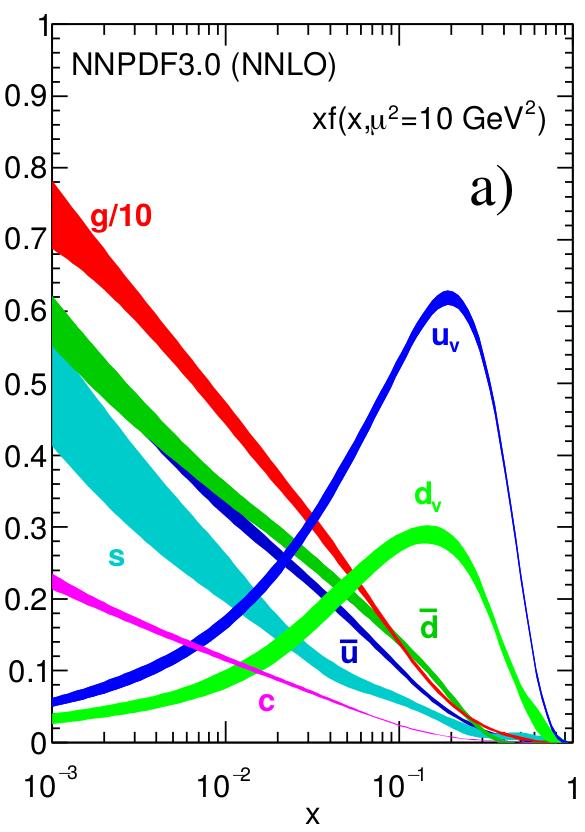
\includegraphics[width=5cm]{\PhDthesisdir/plots_and_images/from_PDG_booklet_2020/parton_pdf_100_GeV2.png}};

% masks
\fill [white] (0,0) rectangle (5,.75);
\fill [white] (0,0) rectangle (.425,7);
\fill [white] (.6,6.7) -- (.6,6) -- (4,5) -- (4.7,5) -- (4.7,6.7);

% X axis
\foreach \pos/\val in {-3/e-3,-2/e-2,-1/e-1,0/1}{
\draw ({4.9+(4.9-.45)*(\pos)/(3)}, .4) node {\footnotesize \num{\val}\vphantom{ÀQg}};
}
\draw (2.7, .2) node {\normalsize $x$};

% Y axis
\foreach \val in {0,0.1,0.2,0.3,0.4,0.5,0.6,0.7,0.8,0.9,1}{
\draw (.5, {.75+\val*(6.9-.75)}) node [left] {\footnotesize \num{\val}};
}

\draw (.5, 6.5) node [right] {\footnotesize NNPDF3.0 (NNLO)};
\draw (4.9,6) node [left] {\scriptsize $x \, f(x, \mu^2=\SI{10}{\GeV^2})$};

\end{tikzpicture}
